% =================================================
% MAIN DOCUMENT (HANDOUT TEMPLATE)
% =================================================
%
% Physics / mathematics handouts and problem sheets.
%
% Typographic appearance is defined in handoutstyle.sty
% and should not be altered here.
%
% =================================================


\documentclass[11pt]{article}


% =================================================
% LOAD HANDOUT STYLE
% =================================================
\usepackage{handoutstyle}


% =================================================
% LANGUAGE
% =================================================
\usepackage[english]{babel}


% =================================================
% CUSTOM PACKAGES
%
% Add project-specific packages here.
% Do not insert packages elsewhere in the file.
% =================================================

% --- Mathematics (defaults) ---
\usepackage{amsmath, amssymb}

% --- Figures ---
\usepackage{graphicx}                % figures
\graphicspath{{figures/}}            % figures live in figures/

% --- Optional ---
% \usepackage{physics}              % \dd, \ket, \bra, ...
% \usepackage{tikz}                 % diagrams


% =================================================
% CUSTOM COMMANDS
%
% Project-specific macros.
%
% The \separator rule is provided by handoutstyle.sty.
% =================================================

% \newcommand{\dd}{\mathrm{d}}
% \newcommand{\Ham}{\mathcal{H}}


% =================================================
% METADATA
% =================================================
\title{Handout Title}
\date{Spring 2026 $\cdot$ Course Name}


% =================================================
% DOCUMENT
% =================================================
\begin{document}

\maketitle


% =================================================
% SECTION
% =================================================
\section{Energy and Conservation}

A particle of mass $m$ moves in a one-dimensional potential
$V(x)$. The total mechanical energy is
\begin{equation}
  E = \tfrac{1}{2} m v^2 + V(x),
\end{equation}
which is conserved when no external forces act.

\begin{definition}
A force is \emph{conservative} if it can be written as the
negative gradient of a potential, $F(x) = -\,\mathrm{d}V/\mathrm{d}x$.
\end{definition}

\begin{theorem}
For a conservative force, the total mechanical energy $E$ is
constant along any solution of the equation of motion.
\end{theorem}

\begin{remark}
The converse fails in general: dissipative systems admit no
such potential, and $E$ is not conserved.
\end{remark}


% =================================================
% EXERCISE
% =================================================
\begin{exercise}[Simple harmonic oscillator]
Consider a particle of mass $m$ in the potential
$V(x) = \tfrac{1}{2}kx^2$.

\begin{subproblems}
  \item Write down the equation of motion using Newton's
        second law.
  \item Show that
        $E = \tfrac{1}{2}mv^2 + \tfrac{1}{2}kx^2$
        is conserved along solutions.
\end{subproblems}

The result can be verified by differentiating $E$ with respect
to time and using the equation of motion from part~(a).

\begin{subproblems}[resume]
  \item Find the angular frequency of small oscillations.
\end{subproblems}
\end{exercise}

\separator


% =================================================
% EXERCISE
% =================================================
\begin{exercise}[Inclined plane]
A block of mass $m$ slides down a frictionless inclined plane
that makes an angle $\theta$ with the horizontal.

\begin{subproblems}
  \item Find the acceleration along the plane.
  \item How long does it take to slide a distance $L$ from rest?
  \item What is the speed at the bottom?
\end{subproblems}
\end{exercise}


% =================================================
% SECTION
% =================================================
\section{Circular Motion}

\begin{figure}[t]
  \centering
  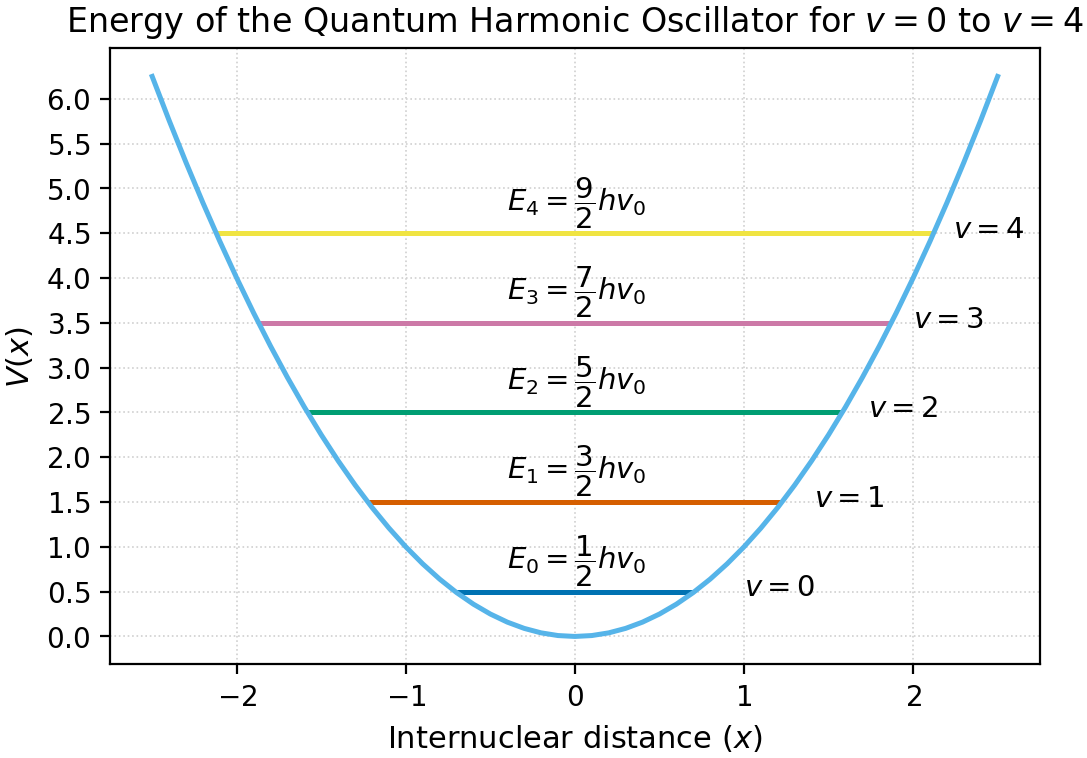
\includegraphics[width=0.5\linewidth]{Energy_levels}
  \caption{Schematic figure for the topic.}
  \label{fig:circular}
\end{figure}

In uniform circular motion, the centripetal acceleration has
magnitude $a_c = v^2/r$, directed toward the center of the
circle.


% =================================================
% EXERCISE
% =================================================
\begin{exercise}[Circular orbit]
A satellite moves in a circular orbit at radius $r$ around a
planet of mass $M$.

\begin{subproblems}
  \item Show that the orbital speed is $v = \sqrt{GM/r}$,
        where $G$ is Newton's gravitational constant.
  \item Express the orbital period $T$ in terms of $r$, $M$,
        and $G$.
\end{subproblems}
\end{exercise}


% =================================================
% SECTION
% =================================================
\section{Numerical Example}

The \verb|python| environment typesets code with Gruvbox Light
syntax highlighting. The short script below verifies the orbital
speed and period from Exercise~3 numerically for three representative
radii.

\begin{python}
import numpy as np

G = 6.674e-11   # gravitational constant  (m^3 kg^-1 s^-2)
M = 5.972e24    # Earth mass              (kg)

orbits = {"Low orbit":    6.40e6,
          "ISS (approx)": 6.78e6,
          "GEO":          4.22e7}

for name, r in orbits.items():
    v = np.sqrt(G * M / r)           # orbital speed  [m/s]
    T = 2 * np.pi * r / v / 3600    # orbital period [hours]
    print(f"{name:14s}  v = {v/1e3:.3f} km/s   T = {T:.2f} h")
\end{python}


\end{document}
